\documentclass[a4paper, 12pt]{article}
\usepackage[utf8]{inputenc}
\usepackage[danish]{babel}
\usepackage{amsmath}
\usepackage{pgfplots}
\pgfplotsset{compat=newest}
\usepackage{amssymb}
\usepackage{siunitx}
\usepackage{fancyhdr}
\usepackage{enumerate}
\usepackage[margin=1in]{geometry}
\title{Opgaver vekselstrøm fysik A}
\author{Christian Kaae Larsen}

\pagestyle{fancy}
\chead{Fysik A}
\rhead{\today}
\lhead{Christian Kaae Larsen, 1. B}

\begin{document}
\maketitle

\section*{Opgave 1}
Find antal vindinger på sekundersiden

Vi kender følgende: \(U_{p}=212 V\) (\(U_{maks})\), \(N_{p}=100\) og \(N_{s}=12 V\)

Vi kender følgende proportion mellem primær og sekundær spoile i en transformer:
\begin{equation*}
	\frac{U_{s}}{U_{p}}=\frac{N_{s}}{N_{p}}
	\label{eq:proportion}
\end{equation*}

For at beregne \(N_{s}\), så skal vi isolere den i formel \eqref{eq:proportion}:

\begin{equation*}
	\frac{U_{s}}{U_{p}}=\frac{N_{s}}{U_{p}} \Leftrightarrow N_{s} = \frac{U_{s}}{U_{p}} \cdot N_{p}
\end{equation*}

Vores \(U_{p}\) er angivet som maksspænding, derfor skal vi lave den om til \(U_{eff}\), da det er det, som vi trækker ud.

\begin{equation*}
	U_{max}=\sqrt{2}\cdot U_{eff} \Leftrightarrow U_{eff}=\frac{U_{max}}{\sqrt{2}}
\end{equation*}

\begin{equation*}
	U_{p} = \frac{212 \si{\volt}}{\sqrt{2}}= 149,9 \si{\volt}
\end{equation*}

Så har vi:
\begin{equation*}
	N_{s}=\frac{12V}{149,9}\cdot 100 = \framebox{8,005}
\end{equation*}

\section*{Opgave 2}
\textit{Find den maksimale effekt, der teoretisk kan opnås ved brug af en nulledning og en fase (fase-0) med en 10A sikring i DK.} \newline

For at beregne effekt anvendes følgende formel:
\begin{equation*}
	P=U \cdot I
\end{equation*}

Vi ved at der spændingensforskellen over en fase og en nulfase i Danmark er \(230 \si{\V}\), så har vi:

\begin{equation*}
	P_{maks}=230 \si{\volt} \cdot 10 \si{\ampere} = \framebox{2300 \si{\watt}}
\end{equation*}

\section*{opgave 3}
\textit{Find den maksimale effekt, der teoretisk kan opnås ved brug af to faseledninger (fase-fase) med en \(16 \si{\ampere}\) sikring i DK} \newline

Vi ved at der i Danmark er en spændingsforskel på \(230 \si{\volt}\) i alle faser.

Så har vi:
\begin{equation*}
	U=230 \si{\volt} \cdot \sqrt{3} = 398 \si{\volt} \approx 400 \si{\volt}  
\end{equation*}

\begin{equation*}
	P_{maks}= U \cdot I = 400 \si{\volt} \cdot 16 \si{\ampere} = \framebox{6400 \si{\watt}}
\end{equation*}

\section*{Opgave 4}
\textit{Find den maksimale effekt, der teoretisk kan opnås ved brug af stjernekoblingen figur 2.} \newline

Vi kan se udfra figur 2. at der på hver af de tre faser (r, s, t) er koblet en \(16 \si{\ampere}\) sikring på. I en stjernekobling er de tre faser koblet på den samme nul-ledning, så hver af de tre faser har den samme effekt, så den maksimale effekt, der kan opnås ved en stjernekobling, må være summen af fasernes effekt: \newline 
For en fase har vi:

\begin{equation*}
	P_{fase} = U \cdot I = 230 \si{\volt} \cdot 10 \si{\ampere} = 2300 \si{\watt} 
\end{equation*}

Så er den samlede maksimale effekt for stjernekoblingen:
\begin{equation*}
	P_{maks} = P_{fase} \cdot 3 = \framebox{6900 \si{\watt}}
\end{equation*}

\section*{Opgave 5}
\textit{Et stykke konstantantråd på \(35 \si{\metre}\) med en diameter på \(0,5 \textrm{mm}\) kobles til en stikkontakt. Bestem den afsatte effekt i tråden.} \newline

For at beregne modstanden i tråden, så skal anvende følgende formel:

\begin{equation*}
	R=\rho \cdot \frac{l}{A}
\end{equation*}

Hvor \(\rho\) er resitiviteten for tråden, \(l\) er længden af tråden og \(A\) er tværsnitsarealet.

Jeg finder konstantantrådens resitivitet ved at slå den op i tabellen på side 116 i Orbit B, hvor den er sat til \(0,490 \frac{\Omega \cdot\textrm{mm}^{2}}{\si{\metre}}\). \newline

Vi ved at trådens diameter er \(0,5 \si{\metre}\), så derfor må tværsnitsarealet \(A\) være:

\begin{equation*}
	A=r^{2} \cdot \pi = \left( \frac{0,5 \textrm{mm}}{2} \right)^{2} \cdot \pi = 0,196 \textrm{mm}^{2}
\end{equation*}

Indsætter de kendte værdier og regner resistensen i tråden:
\begin{equation*}
	R_{konstantan} =\rho \cdot \frac{l}{A} = 0,490 \frac{\Omega \cdot\textrm{mm}^{2}}{\si{\metre}} \cdot \frac{35 \si{\metre}}{0,196 \textrm{mm}^{2}} = 87,5 \si{\ohm}
\end{equation*}

For at beregne tabet anvendes følgende formel:

\begin{equation*}
	P= \frac{U^{2}}{R}
\end{equation*}

Vi ved at spændingsforskellen, som er i en stikkontakt er \(230 \si{\volt}\), derved har vi:

\begin{equation*}
	P_{\textrm{afsat}} = \frac{230 \si{\volt}^{2}}{87,5 \si{\ohm}} = \framebox{604,57 \si{\watt}}
\end{equation*}

\section*{Opgave 6} 

\textit{En \(100 \textrm{L}\) vandvarmer med \(10 \si{\celsius}\) vand kobles til kraft. Varmelegemet er samlet i en stjernekobling som vist på figur 2.} 
\begin{enumerate}[\textbf{a.}]
	\item Hvor lang tid går der før vandet er opvarmet til \(60 \si{\celsius}\)? \newline

	      For at kunne beregne, hvor lang tid det vil tage at opvarme vandet, så skal vi først beregne, hvor meget energi, der skal tilføres vandet for at varme det op til \(60 \si{\celsius}\). For at udregne dette anvendes følgende formel:
	      \begin{equation*}
	      	Q=m \cdot c \cdot \Delta t
	      \end{equation*}
	      
	      Hvor \(Q\) er tilført energi angivet i \(\si{\joule}\), \(m\) er massen, \(c\) er specifik varmekapacitet, som er defineret, som den mængde energi, der skal tilføres et givent materiale for at få det til at stige en grad, og \(\Delta t\) er forøgelsen i temperatur (\(t_{slut}-t_{start}\)). \newline
	      
	      Vands specifikke varmekapacitet er \(4180 \frac{\si{\joule}}{\si{\kilogram} \si{\celsius}}\) ifølge Orbit B. Vi ved, at der opvarmes \(100 \textrm{L}\) vand, så derfor må massen være lig \(100 \si{\kilogram}\), da densiteten for vand er \(1,00 \frac{\si{\gram}}{\textrm{cm}^{3}}\). Ydermere ved vi at vandet opvarmes fra \(10 \si{\celsius}\) til \(60 \si{\celsius}\), derved har vi \(\Delta t = (60 \si{\celsius} - 10 \si{\celsius}) = 50 \si{\celsius}\), så indsætter vi i formel x:
	      
	      \begin{equation*}
	      	Q= 100 \si{\kilogram} \cdot 4180 \frac{\si{\joule}}{\si{\kilogram}  \si{\celsius}} \cdot 50 \si{\celsius} = 2,09 \cdot 10^{7} \si{\joule}
	      \end{equation*}
	      
	      Nu ved vi, hvor meget energi, der anvendes for at varme vandet op. Vi anvender kraft, hvor vi antager at varmelegemet trækker den størst mulige strøm som en \(10 \si{\ampere}\) sikring tillader. I opgave 4 udregnede vi den maksimale effekt, som man kunne trække på et kraft stik, hvor hver fase havde en \(16 \si{\ampere}\) sikring. Her fik vi den maksimale udregnede vi den maksimale effekt til \(6900 \si{\watt}\). Ud fra disse oplysninger kan vi udregne, hvor lang til det vil tage at varme vandet op ved hjælp af kraft, ved at benytte følgende formel:
	      
	      \begin{equation*}
	      	P=\frac{E}{t} \Leftrightarrow  t=\frac{E}{P}= \frac{2,09 \cdot 10^{7} \si{\joule}}{6900 \si{\watt}} \approx \framebox{3029 \si{\second}}
	      \end{equation*}
	\item Hvor lang tid ville det tage at opvarme vandet til \(60 \si{\celsius}\), hvis man blot benyttede et varmelegeme koblet til en almindelig \(230 \si{\volt}\) stikkontakt? \newline
	      
	      Som vi beregnede i opgave 6.a, så krævede det \(2,09 \cdot 10^{7} \si{\joule}\) at opvarme vandet. Det eneste forskel er, at der nu anvendes en stikkontakt fremfor et kraftstik. I opgave 2 udregnede vi den maksimale effekt, der teoretisk set kan trækkes, når der anvendes \(10 \si{\ampere}\) sikringer. I opgave 2 blev den maksimale effekt for stikontakten beregnet til \(2300 \si{\watt}\). Ud fra disse oplysninger kan vi udregne, hvor lang til det vil tage at varme vandet op ved hjælp af en stikkontant, ved at benytte samme formel som i opgave 6.a:
	      \begin{equation*}
	      	t=\frac{E}{P}=\frac{2,09 \cdot 10^{7} \si{\joule}}{2300 \si{\watt}} \approx \framebox{9087 \si{\second}}
	      \end{equation*}
	      
	      Disse to resultater stemmer godt overens fordi, når effekten bliver tredobblet (fra stikkontakten til kraftstikket), så bliver tiden tre gange så kort: \(\frac{9087 \si{\second}} {3029 \si{\second}} = 3 \), så tiden \(t\) og effekten \(P\) må derfor være omvendt proportionale.
\end{enumerate}

\section*{Opgave 7}

\begin{equation*}
	f(t)=A \cdot sin(\omega \cdot t + \varphi)
\end{equation*}

vi kender \(\omega = \frac{2\pi}{T}\), \(\varphi = 2,09\), \(A = 3 V\) \newline
Vi ved at magneterne roterer 15 gange i minuttet, så derfor er deres frekvens: \(\frac{15}{60}=0,25 \textrm{Hz}\). Så kan vi udregne perioden \(T\), og derefter vinkelhastigheden \(\omega\):
\begin{equation*}
	f=\frac{1}{T} \Leftrightarrow T=\frac{1}{f}=\frac{1}{0,25}=4
\end{equation*}

\begin{equation*}
	\omega = \frac{2\pi}{4}=1,57
\end{equation*}
Vi har givet forskydninge \(\varphi\), men den er angivet i \textdegree, så den omregnes til radianer:

\begin{equation*}
	\varphi = \frac{120^{\circ}\cdot \pi}{180^{\circ}}=2,09
\end{equation*}
Så kan vi opstille de tre funktioner for faserne \(L_{1}, L_{2} \ \textrm{og} \ L_{3}\)

\begin{gather*}
	L_{1}(t)=3 \cdot sin(1,57 \cdot t)        \\
	L_{2}(t)=3 \cdot sin(1,57 \cdot t + 2,09) \\
	L_{3}(t)=3 \cdot sin(1,57 \cdot t + 4,18) 
\end{gather*}
	\centering
	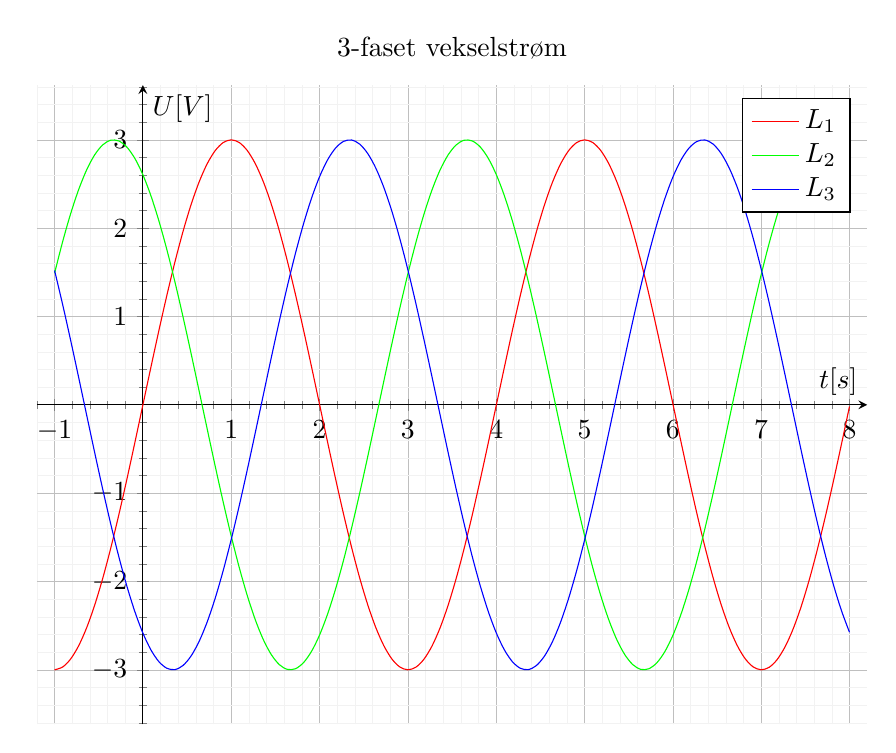
\begin{tikzpicture}
		\begin{axis}%
			[grid=both, xlabel={$t[s]$}, ylabel={$U[V]$}, title={3-faset vekselstrøm}, width=1\textwidth,
				height=0.8\textwidth, 
				minor tick num=4	, axis equal,
				grid style={line width=.1pt, draw=gray!10},
				major grid style={line width=.2pt,draw=gray!50},
				axis lines=middle,
				enlargelimits={abs=0.2}
			]
			\addplot[domain=-1:8,samples=100,smooth,red] {3*sin(deg(1.57*x))};
			\addlegendentry{\(L_{1}\)}
			\addplot[domain=-1:8,samples=100,smooth,green] {3*sin(deg(1.57*x+2.09))};
			\addlegendentry{\(L_{2}\)}
			\addplot[domain=-1:8,samples=100,smooth,blue] {3*sin(deg(1.57*x+2.09*2))};
			\addlegendentry{\(L_{3}\)}
		\end{axis}
	\end{tikzpicture}
\end{document}